% Provenance (never printed): see sources/outline_sources.md (Year 2: the vanished ocean;
% ophiolites; nappes; high-pressure rocks; foreland basins; reconstructing the history from
% maps, sections and geophysics). Units, ages and architecture after Schmid et al. (2004);
% Monte Cervino sheet notes (ISPRA 2016); Penrose definition as quoted by Coleman (1984);
% Zermatt-Saas ages Rubatto et al. (1998), Halama et al. (2020); Chenaillet Corno et al.
% (2023); Moho picks Michailos et al. (2023, Zenodo, CC BY 4.0); gravity Zahorec et al.
% (2021); Jura Lanza et al. (2022), Schori et al. (2015); shortening Rosenberg et al.
% (2021); Glarus thrust Herwegh et al. (2008); Molasse Krenmayr (1999), Garefalakis and
% Schlunegger (2018), Sinclair (1997); present uplift Champagnac et al. (2009). Figure data
% in figdata/bachelor-2/alps.py; exercise and problem values in the Book 4 scratch
% calculator calc/ch13.py.
\chapter{Anatomie d'une chaîne de montagnes~: les Alpes}\label{ch:b2:alpine-orogen}

Le sommet du Cervin est fait de gneiss et de gabbro qui appartenaient autrefois à la marge
de l'Apulie, le continent situé du côté de l'Afrique d'un océan disparu. Les pentes situées
sous lui sont le fond de cet océan, serpentinite, gabbro et basalte en coussins transformés en
éclogite, et plus bas, dans le Mont-Rose voisin, se trouve le bord de l'Europe. En gravissant
la pile, on traverse un continent, puis un océan, puis l'autre. Ce chapitre lit les Alpes comme une telle pile~: d'où viennent ses morceaux, comment ils ont été
empilés, combien de terrain l'empilement a dévoré, et ce que la géophysique voit en profondeur.
% ledger: ispra16:cervino, schmid04:apulia, schmid04:alpine-tethys

\begin{recall}
\textbf{Du volume de lycée}~: collision continentale, suture, raccourcissement d'une
couche (la fraction de sa longueur perdue), failles inverses et chevauchements. \textbf{Du
volume de première année}~: cartes géologiques et coupes~; failles normales, inverses et de chevauchement, plis et
vergence~; marges passives~; croûte océanique, laves en coussins et complexe filonien~;
marges actives et prisme d'accrétion~; isostasie, racine d'Airy et anomalie de Bouguer~;
le \omterm{def:b2:alpine-orogen:foreland}{bassin d'avant-pays}, cité parmi les bassins sédimentaires. \textbf{Du
\cref{ch:b2:metamorphic-facies}}~: les faciès à schistes bleus et à éclogites. \textbf{Du
\cref{ch:b2:pt-paths}}~: \omterm{def:b2:pt-paths:ptt}{chemins P--T--t}, \omterm{def:b2:pt-paths:exhumation}{vitesses d'exhumation} et \omterm{def:b2:metamorphic-facies:metamorphism}{métamorphisme} de
\omterm{def:b2:pt-paths:uhp}{ultra-haute pression}.
\end{recall}

\begin{definition}[Orogène]\label{def:b2:alpine-orogen:orogen}
Un \emph{orogène}\index{orogène} est une bande de lithosphère raccourcie et épaissie par la
convergence de deux plaques, avec les roches déformées et métamorphisées qu'elle contient~; la
chaîne de montagnes en est l'expression en surface, et la croûte épaissie en dessous, sa racine.
\end{definition}

\section{Un océan disparu}\label{sec:b2:alpine-orogen:tethys}

Les Alpes gardent la trace de la fermeture d'océans pendant que les plaques africaine et européenne
convergeaient. Le principal est la \emph{Téthys alpine}, formée de deux branches. Sa
branche méridionale, l'océan Piémont--Ligurie, commença à s'ouvrir au Jurassique moyen, quand
l'Atlantique central s'ouvrait~: la Téthys alpine appartient, par sa cinématique, à l'ouverture de
l'Atlantique, à la différence des océans téthysiens plus à l'est. Les radiolarites, boues siliceuses
des abysses durcies en roche, puis les calcaires à aptychus, succédèrent au début de
l'expansion, et ils signent encore ses vestiges. Une branche septentrionale étroite, l'océan du
Valais, s'ouvrit probablement au tout début du Crétacé. Entre les deux s'étendait une bande continentale, le
Briançonnais, qui s'amincit vers l'est et est absent des Alpes orientales.
% ledger: schmid04:alpine-tethys

Au nord, l'océan était bordé par la marge passive de l'Europe, objet du chapitre sur les rifts et les
marges du volume de première année. Au sud s'étendait l'\emph{Apulie}~: tout le domaine continental situé au sud de la
Téthys alpine et au nord de la plus jeune Néotéthys, y compris l'avant-pays
qui s'étend aujourd'hui au sud des Alpes. Le sommet du Cervin en est un morceau.
% ledger: schmid04:apulia
La carte ci-dessous situe la chaîne et les lieux de ce chapitre.

\begin{omfigure}
\centering
% ledger: data:b4-etopo-alps, schmid04:windows, schmid04:foreland, ispra16:cervino
\begin{tikzpicture}
\begin{axis}[width=0.96\linewidth, height=0.74\linewidth, xmin=5, xmax=14, ymin=43.5,
  ymax=48.5, xlabel={longitude (\unit{\degree} E)}, ylabel={latitude (\unit{\degree} N)},
  tick label style={font=\scriptsize}, label style={font=\small}, clip=true,
  xtick={5,6,...,14}, ytick={44,45,...,48}]
\addplot[omThm!35, line width=0.3pt] table[x=lon, y=lat] {figdata/out/bachelor-2-alps-c1000.dat};
\addplot[omThm!90!black, line width=0.45pt] table[x=lon, y=lat] {figdata/out/bachelor-2-alps-c2000.dat};
\addplot[blue!60!black, line width=0.5pt] table[x=lon, y=lat] {figdata/out/bachelor-2-alps-c0.dat};
\draw[red!70!black, line width=1pt] (axis cs:8,45.3) -- (axis cs:8,48.0);
\node[font=\scriptsize\bfseries, red!70!black, anchor=north west] at (axis cs:8.02,45.32) {A};
\node[font=\scriptsize\bfseries, red!70!black, anchor=south west] at (axis cs:8.02,47.98) {B};
\fill (axis cs:6.865,45.833) circle (1.3pt) node[font=\scriptsize, fill=white, fill opacity=0.85, text opacity=1, inner sep=1pt, anchor=north east] {Mont Blanc};
\fill (axis cs:7.659,45.976) circle (1.3pt) node[font=\scriptsize, fill=white, fill opacity=0.85, text opacity=1, inner sep=1pt, anchor=south east] {Cervin};
\node[font=\scriptsize\itshape, rotate=40] at (axis cs:6.35,46.85) {Jura};
\node[font=\scriptsize\itshape] at (axis cs:9.35,47.65) {bassin molassique};
\node[font=\scriptsize\itshape] at (axis cs:10.0,45.05) {plaine du Pô};
\node[font=\scriptsize\itshape, align=center, fill=white, fill opacity=0.8, text opacity=1, inner sep=1pt] at (axis cs:10.3,46.95) {fenêtre de\\l'Engadine};
\node[font=\scriptsize\itshape, align=center, fill=white, fill opacity=0.8, text opacity=1, inner sep=1pt] at (axis cs:12.6,47.25) {fenêtre du\\Tauern};
\node[font=\scriptsize\itshape] at (axis cs:8.6,43.85) {mer Ligure};
\end{axis}
\end{tikzpicture}
\par\smallskip{\small Les Alpes d'après le modèle de relief ETOPO1, avec des nœuds espacés de
\qty{0.05}{\degree}~: courbes de niveau à \qty{1000}{m} (clair) et à \qty{2000}{m} (foncé), et le littoral. Le
plus haut nœud de cette grille est à \qty{3914}{m}, près du Mont Blanc~; les sommets sont plus hauts,
car un nœud de la grille échantillonne une maille, non un pic. La ligne A--B le long de \qty{8}{\degree} E est
le profil tracé dans la dernière section du chapitre. Les noms de lieux, placés à la main à leurs
positions approximatives.}
\end{omfigure}

Comment connaître un océan disparu~? Par des morceaux de son fond qui ont échappé à la
subduction et ont été pris dans la chaîne de montagnes.

\begin{definition}[Ophiolite~; séquence ophiolitique de Penrose]\label{def:b2:alpine-orogen:ophiolite}
Une \emph{ophiolite}\index{ophiolite} est un assemblage caractéristique de roches mafiques à ultramafiques,
un morceau de lithosphère océanique aujourd'hui retrouvé sur les continents. La \emph{séquence ophiolitique de
Penrose}\index{séquence ophiolitique de Penrose} est l'assemblage complet défini par une conférence
de géologues en 1972~; de bas en haut~:
\begin{enumerate}
\item un complexe ultramafique de \omterm{def:b2:mantle-melting:peridotites}{harzburgite}, de \omterm{def:b2:mantle-melting:peridotites}{lherzolite} et de \omterm{def:b2:mantle-melting:peridotites}{dunite}, souvent avec une
fabrique de déformation acquise à l'état solide~;
\item un complexe gabbroïque, généralement à textures cumulatives~;
\item un complexe de \omterm{def:b2:magma-emplacement:bodies}{dykes} en filons mafiques~;
\item un complexe volcanique mafique, souvent en coussins.
\end{enumerate}
\end{definition}
% ledger: coleman84:penrose

La définition de Penrose fut un consensus, critiqué dès le départ, et reste en général admise.
Sa séquence est l'empilement de la croûte océanique et du manteau supérieur rencontré dans le
volume de première année~: laves en coussins, \omterm{def:b2:magma-emplacement:bodies}{dykes} en filons, gabbro, puis manteau. Les \omterm{def:b2:alpine-orogen:ophiolite}{ophiolites} ne sont cependant pas
un fond océanique ordinaire. La plus grande part de la croûte abyssale, celle des océans larges, est consommée par
la subduction~; Coleman soutint que les \omterm{def:b2:alpine-orogen:ophiolite}{ophiolites} des chaînes alpines et cordillériennes se sont formées surtout aux
centres d'expansion de petits bassins océaniques ou entre des arcs insulaires, et que les \omterm{def:b2:alpine-orogen:ophiolite}{ophiolites} téthysiennes
sont nées là où la croûte continentale s'est amincie le long de marges passives jusqu'à l'ouverture d'un petit
océan.
% ledger: coleman84:penrose, coleman84:settings

Les \omterm{def:b2:alpine-orogen:ophiolite}{ophiolites} alpines entrent dans ce cadre. Les unités issues de l'océan Piémont--Ligurie
sont des reliques de lithosphère océanique et de manteau remonté depuis le dessous du continent aminci,
le manteau sous-continental, puis exposé sur le fond marin. Au Chenaillet, dans les Alpes occidentales,
la plus belle conservée d'entre elles montre du manteau à nu, des gabbros et une célèbre séquence de
basaltes en coussins, sans aucune couverture sédimentaire.
La photographie ci-dessous les montre.
% ledger: schmid04:units, corno23:chenaillet

\begin{omfigure}
\centering
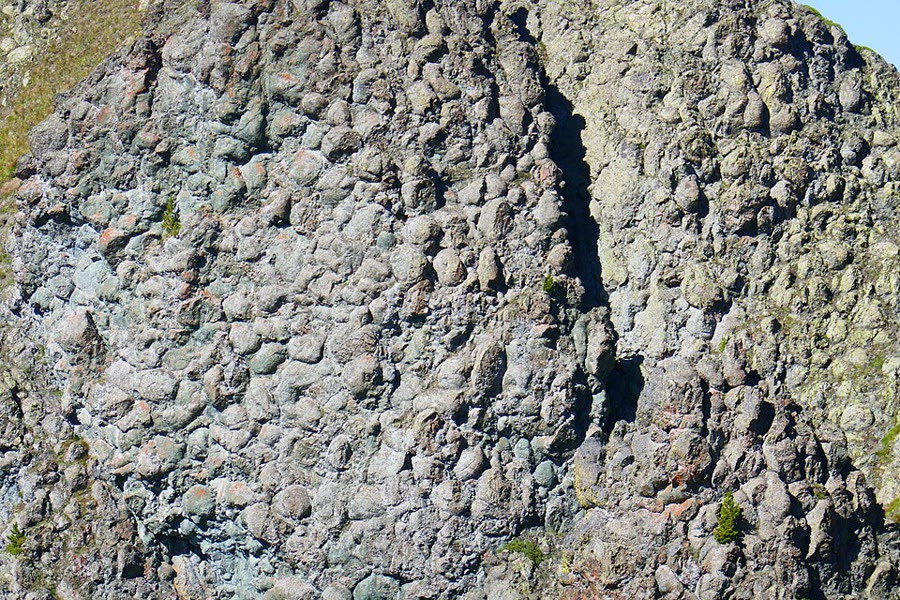
\includegraphics[width=0.66\linewidth]{images/book4/b2-13-pillow-lava.jpg}
\par\smallskip{\small Laves en coussins de l'\omterm{def:b2:alpine-orogen:ophiolite}{ophiolite} du Chenaillet, Alpes occidentales~: chaque
coussin arrondi est un lobe de basalte qui a jailli et s'est refroidi sur le fond de l'océan
Piémont--Ligurie. Photographie Lionel Duchoiselle, CC BY-SA 3.0.}
\end{omfigure}

Le fond océanique peut être daté là où ses gabbros ont cristallisé. Des zircons de deux métagabbros de
l'\omterm{def:b2:alpine-orogen:ophiolite}{ophiolite} de Zermatt--Saas, sous le Cervin, donnent $164.0 \pm \qty{2.7}{Ma}$ et $163.5
\pm \qty{1.8}{Ma}$, et les sédiments riches en manganèse déposés sur les basaltes sont vieux d'au plus $161
\pm \qty{11}{Ma}$ d'âge~: le fond de l'océan Piémont--Ligurie se formait au Jurassique,
il y a environ \qty{164}{Ma}.
% ledger: rubatto98:zsf

\section{Subduction d'un océan, puis d'un continent}\label{sec:b2:alpine-orogen:subduction}

Un océan se referme par subduction. Une partie de son fond finit toutefois au-dessus d'un continent
plutôt que sous lui, et certains continents suivent l'océan dans sa descente.

\begin{definition}[Obduction~; subduction continentale]\label{def:b2:alpine-orogen:obduction}
\emph{Obduction}\index{obduction} est la mise en place d'une écaille de lithosphère océanique sur
une marge continentale, l'\omterm{def:b2:alpine-orogen:ophiolite}{ophiolite} chevauchant le continent. \emph{Subduction
continentale}\index{subduction continentale} est la descente de lithosphère continentale, entraînée
par la plaque océanique qui lui est attachée, dans une zone de subduction, après que l'océan situé devant elle
a été consommé.
\end{definition}

L'\omterm{def:b2:alpine-orogen:obduction}{obduction} s'est produite dans les Dinarides, au sud-est des Alpes~: des \omterm{def:b2:alpine-orogen:ophiolite}{ophiolites} de l'océan jurassique
Vardar, elles-mêmes d'âge jurassique moyen, furent poussées au Jurassique supérieur sur un
prisme d'accrétion et sur la marge de l'Apulie. On a longtemps cru qu'elle avait aussi mis en place
l'\omterm{def:b2:alpine-orogen:ophiolite}{ophiolite} du Chenaillet, car ses roches ne montrent qu'un \omterm{def:b2:metamorphic-facies:metamorphism}{métamorphisme} alpin de très bas degré.
Une étude récente a trouvé des reliques de lawsonite et d'omphacite dans son gabbro et son albitite,
ce qui place son pic alpin entre 10 et \qty{11}{kbar} et entre 340 et
\qty{360}{\celsius}~: le poids d'un \omterm{def:b2:alpine-orogen:nappes}{empilement de nappes} de charriage d'environ 35 à \qty{40}{km} d'épaisseur. Les auteurs
concluent que le Chenaillet a été subduit et non obduit, un rappel que la lecture d'une \omterm{def:b2:alpine-orogen:ophiolite}{ophiolite} repose
autant sur son histoire métamorphique que sur ses roches.
% ledger: schmid04:obduction, corno23:chenaillet

\subsection*{L'océan s'enfonce}

Au Crétacé, la marge méridionale, apulienne, de l'océan Piémont--Ligurie devint une marge active~: sa
fosse se remplit de schistes et de grès, aujourd'hui les schistes calcaires appelés
Bündnerschiefer ou schistes lustrés. Les Alpes orientales gardent aussi la trace d'une collision plus ancienne,
la fermeture d'un golfe d'un autre océan, le Meliata, sur l'Apulie, avec un pic de haute pression vers
\qty{100}{Ma}~: les Alpes sont le produit de deux orogenèses, une crétacée et une
tertiaire.
% ledger: schmid04:two-orogenies

L'\omterm{def:b2:alpine-orogen:ophiolite}{ophiolite} de Zermatt--Saas descendit jusqu'au faciès à éclogite défini au
\cref{ch:b2:metamorphic-facies}~: ses éclogites atteignirent 550 à \qty{600}{\celsius} et 2.5 à
\qty{3.0}{GPa}, et la pression maximale fut atteinte entre 48 et \qty{44}{Ma}. Une tranche
de celle-ci, au lac de Cignana, contient de la coésite et des diamants microscopiques, dans des roches
qui étaient des basaltes et des sédiments de fond océanique~; elle atteignit environ \qty{615}{\celsius}
et \qty{2.8}{GPa}, et ses zircons datent ce point le plus profond à $44.1 \pm \qty{0.7}{Ma}$. Le fond
océanique né il y a \qty{164}{Ma} fut subduit, à l'âge de 120 millions d'années, jusqu'à des profondeurs de
\qty{90}{km} ou plus, puis remonta.
% ledger: halama20:cignana, rubatto98:zsf

\subsection*{Le continent suit}

Une fois l'océan disparu, la marge européenne fut entraînée à sa suite. Les quartzites à coésite du massif
de Dora Maira, rencontrés au \cref{ch:b2:pt-paths}, sont de la croûte continentale venue du côté européen de l'océan,
qui atteignit plus de \qty{90}{km} de profondeur, il y a environ
\qty{35}{Ma}, et revint à la vitesse des plaques. La datation des roches de haute
pression à travers la chaîne donne un ordre~: la marge apulienne elle-même (zone de la Sésia) au
Crétacé supérieur, les \omterm{def:b2:alpine-orogen:ophiolite}{ophiolites} de l'océan Piémont--Ligurie vers \qty{44}{Ma}, la
croûte continentale européenne à la fin de l'Éocène. Rubatto et ses collègues y voient trois épisodes de subduction se succédant dans le temps, du
sud-est au nord-ouest, vers l'Europe.
% ledger: chopin84:coesite, rh01:exhumation, rubatto98:zsf, ispra16:cervino

La collision suivit~: l'océan du Valais, dernière bande océanique, se referma durant l'Éocène moyen à
supérieur, et dès lors la croûte continentale fut empilée sur la croûte continentale.
La figure ci-dessous résume cette succession.
% ledger: schmid04:alpine-tethys

\begin{omfigure}
\centering
\begin{tikzpicture}[x=0.95cm, y=0.78cm, font=\scriptsize]
% (a) rifting and spreading
\begin{scope}[yshift=0cm]
\node[anchor=west, font=\scriptsize\bfseries] at (-0.2,0.75) {(a) Jurassique~: l'océan s'ouvre};
\fill[gray!25] (0,0) -- (3.2,0) -- (3.8,-0.6) -- (0,-0.6) -- cycle;
\fill[gray!25] (6.2,0) -- (10,0) -- (10,-0.6) -- (5.6,-0.6) -- cycle;
\fill[omThm!35] (3.2,0) -- (6.2,0) -- (5.6,-0.6) -- (3.8,-0.6) -- cycle;
\fill[blue!8] (0,0) rectangle (10,0.4);
\draw[thick] (4.7,0) -- (4.7,-0.6);
\node at (1.6,-0.3) {Europe};
\node at (8,-0.3) {Apulie};
\node[align=center] at (4.7,0.2) {dorsale};
\end{scope}
% (b) oceanic subduction
\begin{scope}[yshift=-1.7cm]
\node[anchor=west, font=\scriptsize\bfseries] at (-0.2,0.75) {(b) Crétacé à Éocène~: l'océan est subduit};
\fill[blue!8] (0,0) rectangle (7,0.4);
\fill[gray!25] (0,0) -- (3.0,0) -- (3.6,-0.6) -- (0,-0.6) -- cycle;
\fill[omThm!35] (3.0,0) -- (6.3,0) -- (6.0,-0.5) -- (5.6,-0.95) -- (3.6,-0.6) -- cycle;
\fill[gray!25] (6.3,0) -- (6.6,0.3) -- (10,0.3) -- (10,-0.6) -- (6.4,-0.6) -- cycle;
\fill[omThm!35] (5.6,-0.95) -- (6.0,-0.5) -- (7.4,-1.3) -- (7.2,-1.55) -- cycle;
\fill[orange!40] (6.0,0) -- (6.3,0) -- (6.6,0.3) -- (6.35,0.3) -- cycle;
\draw[-{Latex[length=2mm]}] (7.0,-1.0) -- (7.6,-1.38);
\node at (1.6,-0.3) {Europe};
\node at (8.4,-0.15) {Apulie};
\node[anchor=west] at (7.5,-1.1) {éclogite};
\end{scope}
% (c) continental subduction
\begin{scope}[yshift=-3.95cm]
\node[anchor=west, font=\scriptsize\bfseries] at (-0.2,0.75) {(c) Éocène~: la marge européenne suit};
\fill[gray!25] (0,0) -- (5.6,0) -- (6.2,-0.5) -- (7.4,-1.35) -- (7.1,-1.6) -- (5.6,-0.6) -- (0,-0.6) -- cycle;
\fill[omThm!35] (6.2,0.05) -- (6.6,0.3) -- (6.95,0.3) -- (6.4,-0.2) -- cycle;
\fill[gray!25] (6.6,0.3) -- (10,0.3) -- (10,-0.6) -- (6.9,-0.6) -- (6.4,-0.2) -- (6.95,0.3) -- cycle;
\draw[dashed] (6.6,-0.85) circle (0.22);
\draw (6.82,-0.9) -- (7.6,-1.2);
\node[anchor=west] at (7.6,-1.2) {croûte continentale UHP};
\node at (2.4,-0.3) {Europe};
\node at (8.4,-0.15) {Apulie};
\end{scope}
% (d) collision
\begin{scope}[yshift=-6.65cm]
\node[anchor=west, font=\scriptsize\bfseries] at (-0.2,1.4) {(d) De l'Oligocène à nos jours~: collision, nappes, avant-pays};
\fill[yellow!35] (0.6,0) -- (3.4,0) -- (3.4,-0.3) -- cycle;
\fill[gray!25] (0,-0.3) -- (3.4,-0.3) -- (4.2,0.5) -- (5.2,0.75) -- (6.2,0.55) -- (7.0,0.2) -- (10,0.2)
  -- (10,-0.7) -- (6.6,-0.7) -- (5.4,-1.5) -- (4.0,-1.5) -- (3.2,-0.9) -- (0,-0.9) -- cycle;
\draw (3.4,-0.3) -- (4.5,-1.0);
\draw (4.2,0.5) -- (5.6,-0.4);
\draw (5.2,0.75) -- (6.1,0.1);
\fill[omThm!35] (5.05,0.6) -- (5.55,0.68) -- (5.85,0.32) -- (5.4,0.25) -- cycle;
\fill[yellow!35] (7.0,0.2) -- (9.6,0.2) -- (7.0,-0.1) -- cycle;
\node at (1.4,-0.6) {Europe};
\node at (8.6,-0.3) {Apulie};
\node[anchor=south] at (1.9,0.02) {molasse};
\node at (4.7,-1.25) {racine};
\node[anchor=south west] at (6.25,0.6) {empilement de nappes};
\end{scope}
\end{tikzpicture}
\par\smallskip{\small Histoire schématique des Alpes, sans échelle (lithosphère océanique en rouge,
croûte continentale en gris, prisme d'accrétion en orange, \omterm{def:b2:alpine-orogen:foreland}{bassins d'avant-pays} en jaune).
(a)~L'océan Piémont--Ligurie s'ouvre entre l'Europe et l'Apulie. (b)~Son fond est subduit
sous l'Apulie et transformé en éclogite. (c)~La marge européenne est entraînée à sa suite et
métamorphisée à \omterm{def:b2:pt-paths:uhp}{ultra-haute pression}. (d)~La croûte continentale est empilée en \omterm{def:b2:alpine-orogen:nappes}{nappes de charriage} sur une
racine épaissie, avec des \omterm{def:b2:alpine-orogen:foreland}{bassins d'avant-pays} flexuraux de part et d'autre.}
\end{omfigure}
% ledger: schmid04:alpine-tethys, schmid04:two-orogenies, rubatto98:zsf, schmid04:foreland

\section{Nappes de charriage, klippes et fenêtres}\label{sec:b2:alpine-orogen:nappes}

Les morceaux d'océan et de continent ne furent pas empilés entiers. Ils furent raclés en fines
écailles et transportés très loin.

\begin{definition}[Nappe de charriage~; empilement de nappes]\label{def:b2:alpine-orogen:nappes}
Une \emph{nappe de charriage}\index{nappe de charriage} est une grande feuille de roches, souvent épaisse de
quelques kilomètres et longue de dizaines de kilomètres, transportée le long d'un chevauchement à faible
pendage ou dans le flanc inversé d'un grand pli couché, loin de son lieu d'origine~; les roches d'une nappe sont
\emph{allochtones}\index{allochtone (unité rocheuse)}, celles qui sont restées en place
\emph{autochtones}\index{autochtone (unité rocheuse)}. Un \emph{empilement
de nappes}\index{empilement de nappes} est une pile de nappes dans laquelle les nappes situées plus haut
viennent en général de plus loin à l'intérieur de l'\omterm{def:b2:alpine-orogen:orogen}{orogène}.
\end{definition}

Dans les Alpes, l'ordre d'empilement est la géographie de l'océan disparu retournée,
et les unités sont nommées d'après leur origine (tableau ci-dessous).

\begin{omfigure}
\centering\small
\begin{tabular}{>{\raggedright\arraybackslash}p{0.24\linewidth}|>{\raggedright\arraybackslash}p{0.66\linewidth}}
unité (du haut vers le bas) & origine et roches \\ \hline
\omterm{def:b2:alpine-orogen:nappes}{nappes} austroalpines & marge de l'Apulie au nord de la ligne périadriatique~: socle et couverture
écailles détachées de leur croûte inférieure \\
\omterm{def:b2:alpine-orogen:nappes}{nappes} de Margna--Sesia (zone de la Sésia, Dent Blanche) & fragments détachés de la marge
apulienne la plus externe lors de l'ouverture de l'océan \\
\omterm{def:b2:alpine-orogen:nappes}{nappes} penniques supérieures & océan Piémont--Ligurie~: \omterm{def:b2:alpine-orogen:ophiolite}{ophiolites}, manteau exhumé, schistes
calcaires \\
\omterm{def:b2:alpine-orogen:nappes}{nappes} penniques moyennes & la bande continentale du Briançonnais \\
\omterm{def:b2:alpine-orogen:nappes}{nappes} penniques inférieures & océan du Valais~: \omterm{def:b2:alpine-orogen:ophiolite}{ophiolites} et schistes calcaires \\
\omterm{def:b2:alpine-orogen:nappes}{nappes} subpenniques & socle européen détaché de sa croûte inférieure \\
\omterm{def:b2:alpine-orogen:nappes}{nappes} helvétiques & couverture riche en calcaires de la marge européenne proche, détachée de son
socle \\ \hline
Alpes méridionales & Apulie au sud de la ligne périadriatique~: une \omterm{def:b2:alpine-orogen:ftb}{chaîne plissée et chevauchante} à vergence sud,
surtout miocène, de 10 à \qty{15}{km} d'épaisseur
\end{tabular}
\par\smallskip{\small Les principales unités tectoniques des Alpes, du sommet structural
vers le bas, avec le domaine d'origine de chacune (d'après Schmid et ses collègues).}
\end{omfigure}
% ledger: schmid04:units, schmid04:apulia

La plaque supérieure, l'Apulie, est au sommet~; sous elle viennent, dans l'ordre, l'océan lointain, le
Briançonnais, l'océan proche et la marge européenne, les unités les plus basses étant celles qui étaient les plus
proches de l'Europe. De grands plis, qui ont replissé les \omterm{def:b2:alpine-orogen:nappes}{nappes} après leur empilement, bouleversent parfois l'ordre,
et certaines écailles, comme le Briançonnais, se biseautent le long de la
chaîne.
% ledger: schmid04:units, schmid04:alpine-tethys

L'érosion découpe ensuite l'empilement, et deux formes apparaissent sur une carte.

\begin{definition}[Klippe~; fenêtre tectonique]\label{def:b2:alpine-orogen:klippe}
Une \emph{klippe}\index{klippe} (pluriel~: klippes) est un vestige isolé d'une \omterm{def:b2:alpine-orogen:nappes}{nappe de charriage}, laissé
posé sur les roches sous-jacentes après que l'érosion a emporté le reste de la feuille~; elle est
entourée par son chevauchement de base. Une \emph{fenêtre tectonique}\index{fenêtre tectonique} est un trou
creusé par l'érosion à travers une \omterm{def:b2:alpine-orogen:nappes}{nappe}, où apparaissent les roches situées sous son chevauchement de base, entourées par la
\omterm{def:b2:alpine-orogen:nappes}{nappe}.
\end{definition}

\begin{omfigure}
\centering
\begin{tikzpicture}[x=0.68cm, y=0.68cm, font=\scriptsize]
\def\thrust{(0,0) -- (5,0) .. controls (6.5,0) and (7,1.1) .. (8,1.1)
  .. controls (9,1.1) and (9.5,0) .. (11,0) -- (16,0)}
\def\topo{(0,1.7) .. controls (3,1.9) and (5,1.8) .. (6,1.5) .. controls (7,1.0) .. (8,0.6)
  .. controls (9,1.0) .. (10.3,1.5) .. controls (11.3,1.3) .. (12.5,-0.4)
  .. controls (13.3,0.9) .. (14.5,0.95) .. controls (15.5,0.8) .. (16,-0.2)}
\begin{scope}
\clip \topo -- (16,-2.6) -- (0,-2.6) -- cycle;
\fill[gray!20] (0,-2.6) rectangle (16,2.2);
\fill[omThm!30] \thrust -- (16,2.2) -- (0,2.2) -- cycle;
\draw[gray!55, yshift=-0.9*0.68cm] \thrust;
\draw[gray!55, yshift=-1.8*0.68cm] \thrust;
\draw[line width=1.2pt] \thrust;
\end{scope}
\draw \topo;
\node at (2.5,1.0) {nappe};
\node[anchor=north west] at (0.2,-0.05) {chevauchement de base};
\node at (3.6,-1.35) {autochtone};
\draw[-{Latex[length=1.6mm]}] (8,2.0) node[anchor=south] {fenêtre tectonique} -- (8,0.75);
\draw[-{Latex[length=1.6mm]}] (14.5,2.0) node[anchor=south] {klippe} -- (14.5,1.05);
\end{tikzpicture}
\par\smallskip{\small Une \omterm{def:b2:alpine-orogen:nappes}{nappe} (en couleur) sur son autochtone (gris) après érosion, dans une
coupe schématique~: là où son chevauchement de base (trait épais) se bombe, l'érosion a entaillé
la \omterm{def:b2:alpine-orogen:nappes}{nappe} et ouvert une \omterm{def:b2:alpine-orogen:klippe}{fenêtre tectonique} sur les roches sous-jacentes~; devant, un vestige de la
\omterm{def:b2:alpine-orogen:nappes}{nappe} se dresse isolé sur l'autochtone, une \omterm{def:b2:alpine-orogen:klippe}{klippe}.}
\end{omfigure}

Les Alpes en regorgent. Le Cervin est une \omterm{def:b2:alpine-orogen:klippe}{klippe}~: son sommet appartient au système de chevauchement
de la Dent Blanche, un lambeau de roches apuliennes posé au sommet de tout l'empilement, dont les
gneiss et gabbros d'âge permien reposent sur les \omterm{def:b2:alpine-orogen:ophiolite}{ophiolites} de la \omterm{def:b2:alpine-orogen:nappes}{nappe} de Zermatt--Saas
et de la zone du Combin, qui reposent à leur tour sur les \omterm{def:b2:alpine-orogen:nappes}{nappes} du Mont-Rose et du Grand-Saint-Bernard
du côté européen (photographie ci-dessous). Au front septentrional des Alpes occidentales,
des \omterm{def:b2:alpine-orogen:nappes}{nappes} de couverture venues de loin à l'intérieur de la chaîne forment les Préalpes romandes
et les \omterm{def:b2:alpine-orogen:klippe}{klippes} de la Suisse centrale. Dans les Alpes orientales, deux fenêtres s'ouvrent à travers
le couvercle austroalpin~: la fenêtre de l'Engadine, où les schistes de l'océan du Valais, à schistes bleus,
apparaissent sous les derniers lambeaux du Briançonnais, et la plus grande fenêtre du Tauern, où
la marge européenne et des écailles de la Téthys alpine émergent de sous les \omterm{def:b2:alpine-orogen:nappes}{nappes}
austroalpines.
% ledger: ispra16:cervino, schmid04:windows

\begin{omfigure}
\centering
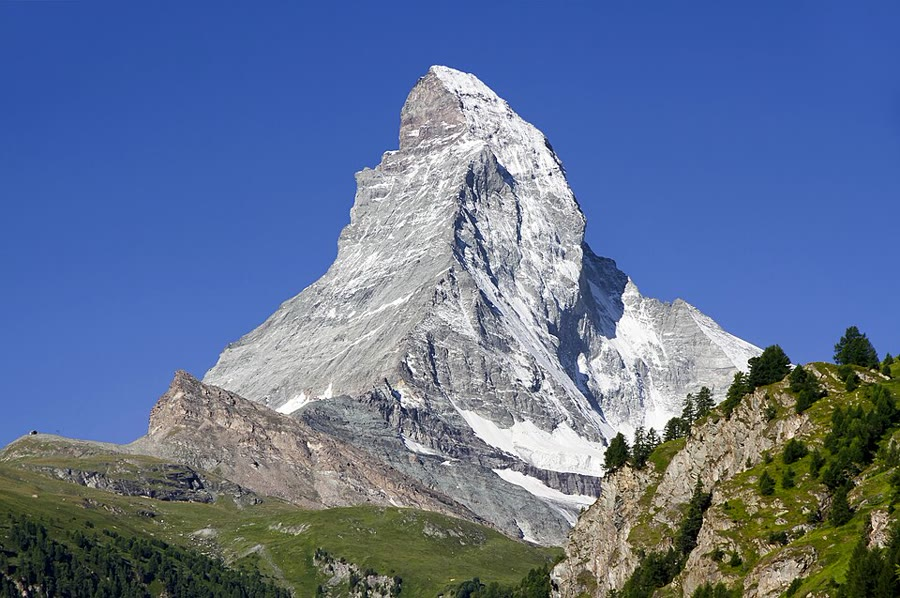
\includegraphics[width=0.7\linewidth]{images/book4/b2-13-matterhorn.jpg}
\par\smallskip{\small Le versant nord-est du Cervin (\qty{4478}{m}), vu de Zermatt~:
sa pyramide supérieure est faite de gneiss et de gabbro apuliens du système de chevauchement de la Dent Blanche, une \omterm{def:b2:alpine-orogen:klippe}{klippe}
sur les \omterm{def:b2:alpine-orogen:ophiolite}{ophiolites} de la Téthys alpine. Photographie Ximonic (Simo Räsänen), CC BY-SA
4.0.}
\end{omfigure}
% ledger: ispra16:cervino

\subsection*{Décollements et les deux peaux}

Les \omterm{def:b2:alpine-orogen:nappes}{nappes} et les écailles de chevauchement se déplacent sur des surfaces de faiblesse.

\begin{definition}[Décollement]\label{def:b2:alpine-orogen:decollement}
Un \emph{décollement}\index{decollement@décollement} est une surface à faible pendage le long de laquelle une
série de roches se détache de celles qui sont dessous et glisse sur elles, les deux côtés se déformant
indépendamment~; elle suit en général une couche faible, telle qu'une évaporite ou une argilite.
\end{definition}

\begin{definition}[Tectonique de couverture et tectonique de socle]\label{def:b2:alpine-orogen:skin}
\emph{Tectonique de couverture}\index{tectonique de couverture} est la déformation d'une
couverture sédimentaire détachée de son socle le long d'un \omterm{def:b2:alpine-orogen:decollement}{décollement} basal~: la couverture se plisse et
chevauche tandis que le socle sous-jacent reste indéformé. \emph{Tectonique
de socle}\index{tectonique de socle} est une déformation dans laquelle le socle est impliqué,
couverture et socle se raccourcissant ensemble, sur des failles qui s'enfoncent dans le socle.
\end{definition}
% ledger: lanza22:jura

\begin{definition}[Chaîne plissée et chevauchante]\label{def:b2:alpine-orogen:ftb}
Une \emph{chaîne plissée et chevauchante}\index{chaîne plissée et chevauchante} est une bande de plis et
de chevauchements qui raccourcit la partie externe d'un \omterm{def:b2:alpine-orogen:orogen}{orogène} et se propage vers son avant-pays~; les
chevauchements remontent du \omterm{def:b2:alpine-orogen:decollement}{décollement} à travers les couches, et les plis croissent au-dessus d'eux.
\end{definition}

Les Alpes ont les deux peaux. Les \omterm{def:b2:alpine-orogen:nappes}{nappes} helvétiques sont une \omterm{def:b2:alpine-orogen:ftb}{chaîne plissée et chevauchante} de couverture, les
calcaires mésozoïques de la marge européenne proche, détachés de leur socle. Leur base est le
chevauchement de Glaris, où les grès rouges permiens reposent sur le \omterm{def:b2:alpine-orogen:foreland}{flysch} cénozoïque. Au Miocène, en
revanche, des blocs du socle européen des massifs externes, raccourcis et épaissis (l'Aar, le
Mont-Blanc, Belledonne, le Pelvoux et l'Argentera), ont été poussés vers le haut avec leur
couverture~: un chevauchement en \omterm{def:b2:alpine-orogen:skin}{tectonique de socle}.
% ledger: schmid04:units, schmid04:skins, herwegh08:glarus, rosenberg21:massifs

Le Jura, l'arc de crêtes au nord-ouest du plateau suisse, est l'exemple classique de \omterm{def:b2:alpine-orogen:skin}{tectonique de
couverture}. Au Miocène supérieur et au Pliocène, sa couverture mésozoïque a été plissée et chevauchée au-dessus d'un
\omterm{def:b2:alpine-orogen:decollement}{décollement} dans les évaporites faibles du Trias moyen et supérieur, tandis que le socle situé dessous,
qui se prolonge depuis les massifs externes sous le bassin molassique, n'a pas été impliqué~: selon la lecture
classique, la poussée venait des massifs externes lointains. La sismologie a depuis ajouté un chapitre de
\omterm{def:b2:alpine-orogen:skin}{tectonique de socle}. Les séismes de Saint-Ursanne en 2000 avaient leur source à moins d'un kilomètre
de profondeur et un mécanisme de chevauchement, un chevauchement superficiel actif dans la couverture,
tandis que d'autres études trouvent des failles du socle réactivées depuis le Pliocène terminal. Savoir si
le Jura est toujours détaché de son socle reste débattu.
% ledger: lanza22:jura, schmid04:skins

\begin{inthefield}[Lire un contact de chevauchement]
Entre Flims et le Walensee, dans l'est de la Suisse, court le chevauchement de Glaris, l'un des
plus importants grands chevauchements à faible pendage des Alpes. Le long de celui-ci, les grès rouges permiens,
le Verrucano, reposent sur le \omterm{def:b2:alpine-orogen:foreland}{flysch} cénozoïque~: des roches bien plus anciennes reposent sur de plus jeunes. Entre les deux, une
mince bande de calcaire fortement cisaillée forme le contact~: le calcaire du Lochseiten, sur lequel le déplacement, d'au moins 30 à
\qty{40}{km}, s'est concentré. Au XIXe siècle, Heim lut la structure comme deux immenses plis couchés
se faisant face~; Escher von der Linth y avait vu un seul chevauchement, et la lecture par chevauchement l'emporta. Un géologue qui rencontre un tel contact vérifie
trois points~: si des roches plus anciennes reposent sur de plus jeunes, ce qu'aucune stratification ordinaire ne peut faire~;
si les couches de part et d'autre sont tronquées au contact~; et si le contact
lui-même est une bande de roche cisaillée et recristallisée plutôt qu'un plan de stratification.
\end{inthefield}
% ledger: herwegh08:glarus

\section{Bassins d'avant-pays~: flysch et molasse}\label{sec:b2:alpine-orogen:foreland}

Une chaîne de montagnes charge la plaque sur laquelle elle repose, et la plaque se courbe vers le bas devant elle.

\begin{definition}[Bassin d'avant-pays~; flysch~; molasse]\label{def:b2:alpine-orogen:foreland}
Un \emph{bassin d'avant-pays}\index{bassin d'avant-pays} est un bassin sédimentaire allongé qui se forme
entre un \omterm{def:b2:alpine-orogen:orogen}{orogène} et le continent stable situé devant lui, là où la plaque est fléchie par la
charge du prisme de chevauchement~; il est le plus profond près du front de chevauchement et est lui-même
progressivement chevauché. Le \emph{flysch}\index{flysch} est le remplissage d'eau profonde d'un tel
bassin, surtout des turbidites de grès et d'argilites déposées tant que le bassin est sous-alimenté.
La \emph{molasse}\index{molasse} est son remplissage ultérieur, marin peu profond et continental, surtout
des conglomérats et des grès issus de la chaîne en érosion, déposés une fois que l'apport remplit le
bassin.
\end{definition}
% ledger: sinclair97:trinity, schmid04:foreland, krenmayr99:molasse

Le fléchissement est une flexure élastique de la lithosphère, traitée dans un chapitre du volume de
troisième année~; ici seul son effet sur le bassin compte. Sinclair décrivit le premier \omterm{def:b2:alpine-orogen:foreland}{bassin d'avant-pays} alpin, d'âge paléocène à oligocène,
comme une «~trinité sous-alimentée~»~: calcaires du côté continental, boues hémipélagiques au
milieu, turbidites d'eau profonde contre le front de chevauchement. À mesure que les chevauchements avançaient, le bassin
suivit leur mouvement~: en Suisse, son rivage continental remontait vers le nord-ouest entre 8.5
et \qty{12.9}{mm} par an, et le bassin migra avec une forme presque constante sur au moins
\qty{210}{km} sur la plaque européenne.
% ledger: sinclair97:trinity

Le bassin molassique nord-alpin, qui s'étend des Alpes-Maritimes à Vienne, commença à s'affaisser à la
fin de l'Éocène. Le \omterm{def:b2:alpine-orogen:foreland}{flysch} de l'Oligocène inférieur, retrouvé aujourd'hui au sommet des \omterm{def:b2:alpine-orogen:nappes}{nappes} helvétiques,
marque un dernier stade d'eau profonde~; de l'Oligocène supérieur au Miocène supérieur, des rivières
étalèrent des graviers et des sables continentaux issus des jeunes montagnes. Le nom est ancien~: H.-B. de Saussure
introduisit le terme \emph{\omterm{def:b2:alpine-orogen:foreland}{molasse}} en 1779. Le remplissage s'épaissit vers la chaîne~: dans le
secteur autrichien, jusqu'à plus de \qty{4000}{m} au front de chevauchement, et ailleurs dans le bassin, une seule
série de conglomérats fluviaux de l'Oligocène supérieur atteint environ \qty{4}{km} d'épaisseur. La partie
méridionale du bassin a été chevauchée~: la bande d'affleurement autrichienne, large d'environ \qty{60}{km}, représente moins
du quart de la largeur ancienne du bassin. La \omterm{def:b2:alpine-orogen:foreland}{molasse} chevauchée elle-même est prise dans les
chevauchements, sous forme de \omterm{def:b2:alpine-orogen:foreland}{molasse} subalpine, des tranches de conglomérat pendant vers le sud le long du
bord septentrional de la chaîne.
% ledger: schmid04:foreland, krenmayr99:molasse, gs18:conglomerates

Au sud des Alpes, la plaine du Pô repose sur l'avant-pays adriatique peu déformé des Alpes
méridionales. Ses sédiments les plus jeunes, pliocènes et pléistocènes, recouvrent en partie les structures alpines
en discordance et sont en partie déformés par les derniers chevauchements des Alpes méridionales
et des Apennins.
% ledger: schmid04:foreland

\begin{omfigure}
\centering
\begin{tikzpicture}[x=0.5cm, y=0.6cm, font=\scriptsize]
\begin{scope}
\node[anchor=west, font=\scriptsize\bfseries] at (0,2.4) {(a) sous-alimenté~: flysch};
\fill[blue!8] (0,0) -- (12,0) -- (12,1.4) -- (9.0,1.4) -- (4,0.05) -- (0,0.05) -- cycle;
\fill[gray!25] (0,0) -- (12,-1.1) -- (12,-1.9) -- (0,-0.8) -- cycle;
\fill[omThm!30] (9.0,1.4) -- (12,2.2) -- (12,-1.1) -- (9.5,-0.87) -- cycle;
\fill[green!25!gray!40] (5.5,-0.5) -- (9.5,-0.87) -- (9.3,-0.35) -- (7.0,-0.2) -- cycle;
\node at (10.9,0.6) {prisme};
\node at (2,-0.45) {craton};
\node[anchor=north] at (7.3,-0.9) {turbidites};
\draw[->] (7.3,-0.95) -- (7.6,-0.55);
\end{scope}
\begin{scope}[xshift=6.4cm]
\node[anchor=west, font=\scriptsize\bfseries] at (0,2.4) {(b) suralimenté~: molasse};
\fill[gray!25] (0,0) -- (12,-1.1) -- (12,-1.9) -- (0,-0.8) -- cycle;
\fill[omThm!30] (8.5,1.6) -- (12,2.4) -- (12,-1.1) -- (9.0,-0.82) -- cycle;
\fill[yellow!40] (1.5,-0.13) -- (9.0,-0.82) -- (8.5,1.0) -- (5,0.35) -- cycle;
\fill[blue!8] (0,0) -- (1.5,-0.13) -- (5,0.35) -- (4,0.4) -- (0,0.4) -- cycle;
\node at (10.6,0.6) {prisme};
\node at (2,-0.45) {craton};
\node at (6.2,-0.05) {graviers, sables};
\end{scope}
\end{tikzpicture}
\par\smallskip{\small Un \omterm{def:b2:alpine-orogen:foreland}{bassin d'avant-pays} en deux étapes (schématique). (a)~Au début, la plaque fléchie
s'affaisse plus vite que n'arrivent les sédiments~: eau profonde contre le prisme de chevauchement, où
s'accumulent les turbidites (\omterm{def:b2:alpine-orogen:foreland}{flysch}). (b)~Plus tard, la chaîne en érosion fournit plus que ce que le bassin peut
contenir~: des rivières le comblent de graviers et de sables (\omterm{def:b2:alpine-orogen:foreland}{molasse}), et le prisme chevauche ses propres
débris.}
\end{omfigure}
% ledger: sinclair97:trinity, schmid04:foreland

\section{Lire l'histoire~: coupes et géophysique}\label{sec:b2:alpine-orogen:sections}

Une carte montre où se trouvent les unités~; une coupe montre comment elles se disposent en profondeur, et elle
peut être testée.

\begin{definition}[Coupe équilibrée]\label{def:b2:alpine-orogen:balanced}
Une \emph{coupe équilibrée}\index{coupe équilibrée} est une coupe de roches déformées, tracée parallèlement à la
direction de transport, qui peut être restaurée dans un état non déformé géologiquement raisonnable
sans gain ni perte de roche~: les longueurs des niveaux repères et
les aires des unités rocheuses de la coupe se conservent entre l'état déformé et l'état
restauré.
\end{definition}

La restauration est ancrée par des \emph{lignes d'ancrage}, lignes traversant les couches aux extrémités de la
coupe, choisies là où les roches n'ont pas glissé les unes contre les autres.

\begin{proposition}[Équilibre des longueurs et des aires]\label{prop:b2:alpine-orogen:balance}
Entre deux lignes d'ancrage distantes de $l$ dans l'état déformé, soit un niveau repère de
longueur $l_0$ mesurée le long du niveau, et une couche d'épaisseur initiale $t$ une aire
de section $A$. Si la longueur et l'aire se conservent dans le plan de la coupe,
\begin{enumerate}
\item le niveau mesurait $l_0$ avant la déformation, le raccourcissement vaut
$e = 1 - l/l_0$ et la distance de raccourcissement $S = l_0 - l$~;
\item la longueur restaurée de la couche est $l_0 = A/t$~;
\item si un horizon repère se trouve à une profondeur $d$ au-dessus d'un \omterm{def:b2:alpine-orogen:decollement}{décollement} plat, l'aire de roche
soulevée au-dessus du niveau initial du repère, son \emph{aire excédentaire} $A_e$, vaut $S\,d$~;
d'où $d = A_e/S$.
\end{enumerate}
\end{proposition}

\begin{omfigure}
\centering
% book's own geometry (figdata/bachelor-2/alps.py)
\begin{tikzpicture}
\begin{axis}[width=0.86\linewidth, height=4.0cm, axis equal image, xmin=-1.5, xmax=31.5,
  ymin=-7.5, ymax=4.8, axis lines=none, clip=false]
\addplot[omThm, line width=1.2pt] table[x=x_km, y=y_km] {figdata/out/bachelor-2-alps-chevron.dat};
\addplot[gray, line width=1.2pt] table[x=x_km, y=y_km] {figdata/out/bachelor-2-alps-chevron0.dat};
\draw[dashed] (axis cs:0,-7) -- (axis cs:0,4.3);
\draw[dashed] (axis cs:22.98,-1.2) -- (axis cs:22.98,4.3);
\draw[dashed] (axis cs:30,-7) -- (axis cs:30,-4.8);
\draw[<->] (axis cs:0,-1.4) -- node[below, font=\scriptsize] {$l = \qty{23.0}{km}$} (axis cs:22.98,-1.4);
\node[font=\scriptsize, anchor=south] at (axis cs:15,-5.9) {restauré~: $l_0 = \qty{30.0}{km}$};
\node[font=\scriptsize, anchor=west] at (axis cs:23.3,2.2) {pendage des flancs \qty{40}{\degree}};
\node[font=\scriptsize, anchor=south] at (axis cs:0,4.3) {ancrage};
\node[font=\scriptsize, anchor=south] at (axis cs:22.98,4.3) {ancrage};
\end{axis}
\end{tikzpicture}
\par\smallskip{\small Équilibre des longueurs d'un niveau repère plié en chevrons, à flancs
pentés de \qty{40}{\degree} (en haut), et le même niveau restauré entre ses lignes d'ancrage
(en bas), à l'échelle réelle. Chaque flanc garde sa longueur~; le niveau plié couvre
$l = 30.0\cos\qty{40}{\degree} = \qty{23.0}{km}$, soit un raccourcissement de $1 - \cos\qty{40}{\degree} =
\qty{23.4}{\percent}$.}
\end{omfigure}

\begin{proof}
(1) Un niveau qui ne s'étire ni ne se raccourcit le long de sa longueur la conserve~; le raccourcissement est
la fraction de longueur perdue, comme à l'école. (2) Avant la déformation, la couche est une bande de
longueur $l_0$ et d'épaisseur $t$, d'aire $l_0 t$, et l'aire se conserve. (3) Avant
la déformation, la roche comprise entre le niveau du repère et le \omterm{def:b2:alpine-orogen:decollement}{décollement} remplissait une bande de longueur $l_0$
et d'épaisseur $d$. Après elle, entre les lignes d'ancrage, la même roche remplit une bande de longueur $l$
depuis le \omterm{def:b2:alpine-orogen:decollement}{décollement} jusqu'au niveau initial du repère, d'aire $l\,d$, plus l'excédent
d'aire repoussée au-dessus de ce niveau. La conservation donne $l_0 d = l\,d + A_e$, donc $A_e = (l_0 -
l)\,d = S\,d$. La relation donne la profondeur d'un \omterm{def:b2:alpine-orogen:decollement}{décollement} caché à partir d'une aire excédentaire
mesurée et du raccourcissement.
\end{proof}


\begin{method}[Restauration d'une coupe]\label{met:b2:alpine-orogen:restore}
\begin{enumerate}
\item Choisir une coupe parallèle à la direction de transport et deux lignes d'ancrage là où il n'y
avait pas de glissement entre les couches.
\item Mesurer chaque niveau repère le long de sa longueur entre les ancrages, en comptant chaque partie
répétée par un chevauchement.
\item Étaler les niveaux à plat à leurs longueurs mesurées, en gardant l'ordre des couches,
et retracer les failles sur la coupe restaurée~: leurs coupures doivent se raccorder, sans lacunes
ni chevauchements.
\item Comparer~: les niveaux d'une même écaille de chevauchement doivent se restaurer à la même longueur~; les aires des
couches, divisées par leurs épaisseurs, doivent donner elles aussi les mêmes longueurs. Une coupe qui
échoue n'est pas admissible telle qu'elle est tracée.
\end{enumerate}
\end{method}

L'équilibrage est un test d'une coupe, non une preuve, et ses hypothèses comptent. Dans le Jura, près du
Chasseral, l'équilibrage des longueurs au toit du Jurassique donne \qty{5.1}{km} de
déplacement, mais l'équilibrage des aires et la modélisation directe donnent \qty{11.3}{km}~: les
\qty{6.2}{km} supplémentaires ont été transportés le long d'un second \omterm{def:b2:alpine-orogen:decollement}{décollement}, supérieur, dans les argilites jurassiques, et transmis
aux plis plus au nord. Un seul niveau repère avait manqué la moitié du mouvement. La même étude
examina, sans en avoir besoin, deux autres interprétations courantes dans le Jura~: des hauts de socle poussant
les plis vers le haut, et des cœurs d'anticlinaux épaissis par des évaporites triasiques qui y fluent, un
processus qui met en défaut l'équilibrage des aires, puisque la couche d'évaporites ne conserve plus son
épaisseur.
% ledger: schori15:chasseral, schori15:evaporite-flow

\subsection*{Quel raccourcissement~?}

Appliqué à des transects entiers, l'équilibrage donne le raccourcissement global de la chaîne, et les réponses
varient avec les hypothèses. Dans les Alpes centrales, le long du transect NFP-20, les estimations
du raccourcissement collisionnel sont d'environ \qty{125}{km} dans les travaux anciens, \qty{160}{km} dans
une compilation de 2015 et \qty{144}{km} dans une synthèse de 2021~; en ajoutant le décrochement dextre de la ligne périadriatique, qui
a déplacé l'Apulie latéralement le long de la chaîne, la convergence globale atteint entre 206 et
\qty{250}{km}, selon le décrochement supposé. Dans les Alpes occidentales, les estimations vont de 124 à
\qty{243}{km}. Chacune d'elles est une somme de morceaux restaurés, chacun avec ses propres lignes
d'ancrage et ses propres suppositions sur ce que l'érosion et la subduction ont retiré.
% ledger: rosenberg21:shortening

\subsection*{Ce que voit la géophysique}

Les coupes en profondeur reposent sur la géophysique. Des profils de sismique réflexion profonde ont été tirés
à travers la chaîne (ECORS--CROP dans les Alpes occidentales, NFP-20 ouest et est en Suisse,
TRANSALP à l'est), et des réseaux denses de sismomètres cartographient désormais le Moho
à partir des fonctions récepteur, c'est-à-dire des conversions d'ondes P télésismiques en ondes S
à la base de la croûte. La carte d'AlpArray, construite à partir de plus de cent mille fonctions récepteur,
situe le Moho
vers \qty{30}{km}, valeur typique des continents, autour de la chaîne, et à 55 à
\qty{60}{km} sous les Alpes~; le Moho européen plonge doucement d'environ \qty{30}{km}
au nord-ouest jusqu'à environ \qty{55}{km} sous la chaîne. La coupe schématique ci-dessous résume comment on lit
les profils NFP-20 à travers les Alpes centrales.
% ledger: schmid04:transects, michailos23:moho

\begin{omfigure}
\centering
\begin{tikzpicture}[x=0.6cm, y=0.5cm, font=\scriptsize]
% surface and cover
\fill[yellow!30] (0,0) -- (3.0,0) -- (6.5,-0.3) -- (8.0,0.4) -- (8.0,-0.9) -- (0,-0.6) -- cycle;
\fill[gray!12] (0,-0.6) -- (8.0,-0.9) -- (12.5,-4.5) -- (15,-3.5) -- (16.5,-6.6) -- (16,-8.3)
  -- (0,-5.0) -- cycle;
\fill[gray!35] (0,-5.0) -- (16,-8.3) -- (17.5,-10.0) -- (0,-6.0) -- cycle;
% Helvetic and Aar
\fill[cyan!25] (8.0,0.4) -- (10.0,1.6) -- (11.0,1.2) -- (9.5,-0.4) -- (8.0,-0.9) -- cycle;
\fill[gray!12] (8.0,-0.9) -- (9.5,-0.4) -- (11.0,1.2) -- (12.0,2.0) -- (12.8,0.2) -- (11.5,-1.8)
  -- (12.5,-4.5) -- cycle;
% Penninic stack
\fill[omThm!35] (12.0,2.0) -- (14.5,2.6) -- (17.0,2.2) -- (17.3,-1.0) -- (15.0,-3.5) -- (12.5,-4.5)
  -- (11.5,-1.8) -- (12.8,0.2) -- cycle;
% Austroalpine/Apulia and Southern Alps
\fill[orange!30] (17.0,2.2) -- (19.0,1.6) -- (24,0.2) -- (26,0) -- (26,-3.5) -- (20.5,-4.0)
  -- (17.3,-1.0) -- cycle;
\fill[brown!35] (17.3,-1.0) -- (20.5,-4.0) -- (19.0,-7.0) -- (16.5,-6.6) -- (15,-3.5) -- cycle;
\fill[gray!35] (20.5,-4.0) -- (26,-3.5) -- (26,-6.0) -- (19.0,-7.0) -- cycle;
\fill[yellow!30] (23.5,0.3) -- (26,0) -- (26,-0.5) -- (24.5,-0.3) -- cycle;
\draw[thick] (17.3,-1.0) -- (17.0,2.2);
\draw[thick] (8.0,-0.9) -- (12.5,-4.5);
\draw[dashed] (0,-6.0) -- (17.5,-10.0);
\draw[dashed] (19.0,-7.0) -- (26,-6.0);
\node at (2.2,-0.25) {Jura};
\node at (5.2,-0.35) {molasse};
\node at (9.0,0.15) {Helvétique};
\node at (10.6,-0.6) {Aar};
\node at (14.6,0.4) {nappes penniques};
\node at (21.2,-0.9) {Alpes méridionales};
\node at (24.9,-0.3) {Pô};
\node at (18.0,-4.8) {Ivrée};
\node[align=center] at (5,-3.0) {croûte européenne};
\node[anchor=north] at (3.2,-7.4) {Moho européen};
\node at (10,-9.3) {manteau};
\node at (23,-7.7) {manteau};
\node[anchor=north] at (23,-6.55) {Moho adriatique};
\node[anchor=south, align=center] at (17.2,2.25) {ligne\\périadriatique};
\draw[-{Latex[length=2mm]}] (1.0,0.5) -- (0.0,0.5);
\node[anchor=south] at (0.5,0.5) {NO};
\draw[-{Latex[length=2mm]}] (25.0,1.2) -- (26.0,1.2);
\node[anchor=south] at (25.5,1.2) {SE};
\end{tikzpicture}
\par\smallskip{\small Coupe crustale schématique à travers les Alpes centrales, du Jura à la plaine
du Pô (sans échelle~; d'après les interprétations des transects NFP-20 compilées par Schmid
et ses collègues). La croûte européenne, avec le Jura replié à son sommet, plonge sous les \omterm{def:b2:alpine-orogen:nappes}{nappes}
helvétiques, le massif de l'Aar et l'\omterm{def:b2:alpine-orogen:nappes}{empilement des nappes} penniques~; au sud de la ligne
périadriatique, la croûte apulienne, avec le coin du corps d'Ivrée, repose sur le Moho européen, et
les Alpes méridionales chevauchent vers le sud la plaine du Pô.}
\end{omfigure}
% ledger: schmid04:transects, schmid04:units, schmid04:apulia, schmid04:skins


\begin{omfigure}
\centering
% ledger: data:b4-etopo-alps, data:b4-alps-moho, michailos23:moho
\begin{tikzpicture}
\begin{groupplot}[group style={group size=1 by 2, vertical sep=0.25cm, x descriptions at=edge bottom},
  width=0.92\linewidth, xmin=0, xmax=300, tick label style={font=\scriptsize},
  label style={font=\small}]
\nextgroupplot[height=3.6cm, ymin=0, ymax=4000, ylabel={altitude (\unit{m})},
  ytick={0,1000,2000,3000,4000}, y tick label style={/pgf/number format/1000 sep={}},
  legend style={font=\scriptsize, at={(0.99,0.97)}, anchor=north east, draw=none, fill=none}]
\addplot[gray, line width=0.4pt] table[x=km, y=max_m] {figdata/out/bachelor-2-alps-swath.dat};
\addplot[omThm, line width=1pt] table[x=km, y=mean_m] {figdata/out/bachelor-2-alps-swath.dat};
\legend{maximum de la bande, moyenne de la bande}
\node[font=\scriptsize, anchor=south west] at (axis cs:2,2650) {A (plaine du Pô)};
\node[font=\scriptsize, anchor=south east] at (axis cs:298,1500) {B};
\nextgroupplot[height=4.6cm, ymin=0, ymax=70, y dir=reverse, xlabel={distance au nord de
  \qty{45.3}{\degree} N le long de \qty{8}{\degree} E (\unit{km})}, ylabel={profondeur (\unit{km})},
  legend style={font=\scriptsize, at={(0.99,0.03)}, anchor=south east, draw=none, fill=none}]
\addplot[only marks, mark=*, mark size=1.6pt, black] table[x=km, y=moho_km] {figdata/out/bachelor-2-alps-moho.dat};
\addplot[omThm, dashed, line width=0.8pt] table[x=km, y=airy_km] {figdata/out/bachelor-2-alps-airy.dat};
\addplot[gray, densely dotted] coordinates {(0,30) (300,30)};
\legend{pointés du Moho, prédiction d'Airy, \qty{30}{km}}
\end{groupplot}
\end{tikzpicture}
\par\smallskip{\small Profil A--B le long de \qty{8}{\degree} E. En haut~: altitude moyenne et maximale des
nœuds ETOPO1 dans une bande de \qty{0.25}{\degree} de part et d'autre du méridien. En bas~: les profondeurs
du Moho pointées sur ce méridien dans la carte des fonctions récepteur d'AlpArray
(Michailos et ses collègues, CC BY 4.0), et le Moho que l'isostasie locale d'Airy placerait sous le relief
moyen de la bande, pour une croûte de \qty{30}{km} et des densités 2700 et
\qty{3300}{kg.m^{-3}}.}
\end{omfigure}

Le profil ci-dessus confronte la racine au modèle d'Airy du volume de première
année. Sous la partie la plus haute du profil, là où le relief moyen de la bande atteint
\qty{2.74}{km} à \qty{46.5}{\degree} N, une racine d'Airy locale placerait le Moho à
$30 + 4.5 \times 2.74 = \qty{42.3}{km}$~; il est observé à \qty{36.3}{km}. Une centaine de
kilomètres plus au sud, au bord de la plaine du Pô, où le relief moyen n'est que
\qty{0.65}{km}, le Moho observé est le plus profond du profil, \qty{61.2}{km}. La racine n'est pas sous les sommets~: elle est
déplacée vers l'Apulie. Sur le tronçon où existent des pointés, sa section, mesurée
sous \qty{30}{km}, est d'environ \qty{2300}{km^2}, contre environ \qty{1500}{km^2} pour les racines d'Airy
du relief qui la surmonte. La compensation locale de la topographie actuelle n'explique pas
la racine. Pfiffner et ses collègues évoquent une charge supplémentaire~: le corps d'Ivrée, un coin de
manteau et de croûte inférieure adriatiques au sein de la chaîne, qui a contribué à fléchir la plaque européenne
vers le bas.
% ledger: data:b4-etopo-alps, data:b4-alps-moho, michailos23:moho, pfiffner02:ivrea

La gravimétrie raconte la même histoire autrement. La carte de l'anomalie de Bouguer panalpine montre une
anomalie négative alpine de $-100$ à \qty{-170}{mGal} le long de la chaîne, la plus forte dans les Alpes centrales,
due à la croûte légère de la racine épaissie~; une dépression du bassin du Pô d'environ $-80$ à
\qty{-140}{mGal}~; et, entre les Alpes occidentales et la plaine du Pô, l'étroit maximum gravimétrique d'Ivrée
culminant à \qty{+40}{mGal}, là où cette croûte inférieure et ce manteau denses approchent de la
surface.
% ledger: zahorec21:gravity

\section{Une chronologie des Alpes}\label{sec:b2:alpine-orogen:timeline}

Rassembler les dates de ce chapitre donne l'histoire de la chaîne en un seul tableau
(tableau ci-dessous).

\begin{omfigure}
\centering\small
\begin{tabular}{p{0.28\linewidth}|p{0.62\linewidth}}
temps & événement \\ \hline
Jurassique moyen & l'océan Piémont--Ligurie s'ouvre~; ses gabbros cristallisent à
\qty{164}{Ma} \\
Crétacé le plus ancien & l'océan du Valais s'ouvre au nord du Briançonnais \\
vers \qty{100}{Ma} & pic de haute pression de l'orogenèse crétacée dans les Alpes orientales \\
Crétacé supérieur & la marge apulienne (zone de la Sésia) est subduite~; la marge apulienne de
l'océan est active \\
de 48 à \qty{44}{Ma} & le fond océanique de Zermatt--Saas atteint son point le plus profond, coésite et
diamant au lac de Cignana \\
de l'Éocène moyen à supérieur & l'océan du Valais se referme~; le bassin molassique commence à s'affaisser \\
\qty{35}{Ma} & croûte continentale de Dora Maira à \omterm{def:b2:pt-paths:uhp}{ultra-haute pression} \\
Oligocène et Miocène & le chevauchement de Glaris~; les graviers molassiques remplissent l'avant-pays nord (de
l'Oligocène supérieur au Miocène supérieur) \\
Miocène & soulèvement en \omterm{def:b2:alpine-orogen:skin}{tectonique de socle} des massifs externes~; les Alpes méridionales chevauchent
vers le sud \\
du Miocène supérieur au Pliocène & plissement en \omterm{def:b2:alpine-orogen:skin}{tectonique de couverture} du Jura \\
aujourd'hui & le nivellement montre un soulèvement relatif des roches pouvant atteindre \qty{1.3}{mm} par an au cœur de
les Alpes centrales
\end{tabular}
\par\smallskip{\small Les Alpes en onze étapes~; les sources sont citées dans les sections
ci-dessus.}
\end{omfigure}
% ledger: schmid04:alpine-tethys, rubatto98:zsf, schmid04:two-orogenies, halama20:cignana, schmid04:foreland, rh01:exhumation, herwegh08:glarus, schmid04:skins, schmid04:apulia, champagnac09:uplift

La dernière ligne n'est pas la fin de la convergence. Des nivellements répétés à travers les Alpes centrales
donnent un soulèvement relatif des roches allant d'environ \qty{-0.4}{mm} par an au nord du Jura à
\qty{1.3}{mm} par an au cœur de la chaîne, tandis que les mesures GPS suggèrent que les Alpes
centrales ne convergent plus aujourd'hui. Champagnac et ses collègues lisent ce soulèvement comme le rebond isostatique d'une
croûte déchargée par l'érosion~: les montagnes s'élèvent parce qu'elles sont usées.
% ledger: champagnac09:uplift

\section*{Exercices}\label{sec:b2:alpine-orogen:exercises}

Données~: $g = \qty{9.8}{m.s^{-2}}$,
$G = \qty{6.674e-11}{m^3.kg^{-1}.s^{-2}}$.

\begin{exercise}[$\star$]\label{exo:b2:alpine-orogen:1}
Dans une coupe, un niveau calcaire mesuré le long de ses plis entre deux lignes d'ancrage mesure
\qty{36.0}{km} de long~; les lignes d'ancrage sont distantes de \qty{27.0}{km}. (a) En utilisant
\cref{prop:b2:alpine-orogen:balance}, calculer le raccourcissement $e$ et la distance de raccourcissement
$S$. (b) Quelle condition le niveau doit-il remplir pour que la réponse soit valable~?
\end{exercise}

\begin{exercise}[$\star$]\label{exo:b2:alpine-orogen:2}
Sur une carte géologique, (a) une tache ovale de gneiss longue de \qty{4}{km} repose sur du calcaire
jurassique, dont la limite est un chevauchement plongeant vers l'intérieur, sous le gneiss, tout autour~; (b) une
zone allongée d'argilite crétacée est entourée de gneiss, le long d'un chevauchement plongeant vers
l'extérieur, sous le gneiss, tout autour. Nommer chaque structure et dire ce que l'érosion en a fait
dans chaque cas.
\end{exercise}

\begin{exercise}[$\star$]\label{exo:b2:alpine-orogen:3}
(a) Énumérer les quatre unités de la \omterm{def:b2:alpine-orogen:ophiolite}{séquence ophiolitique de Penrose}, de bas en haut, et associer chacune
à une couche de la croûte océanique ou du manteau. (b) L'\omterm{def:b2:alpine-orogen:ophiolite}{ophiolite} du Chenaillet montre du manteau à nu,
des gabbros et des basaltes en coussins, et aucune couverture sédimentaire. Quelle unité de Penrose cette liste
omet-elle~? (c) Pourquoi les \omterm{def:b2:alpine-orogen:ophiolite}{ophiolites} ne donnent-elles pas un échantillon fidèle du fond des
océans larges~?
\end{exercise}
% ledger: coleman84:penrose, coleman84:settings, corno23:chenaillet

\begin{exercise}[$\star$]\label{exo:b2:alpine-orogen:4}
En montant au Cervin par le sud, un alpiniste traverse tour à tour les \omterm{def:b2:alpine-orogen:nappes}{nappes} du Mont-Rose et du
Grand-Saint-Bernard, les \omterm{def:b2:alpine-orogen:ophiolite}{ophiolites} de Zermatt--Saas, la zone du Combin et les gneiss du système de
chevauchement de la Dent Blanche. (a) Donner le domaine d'origine de chacune. (b) Quelle plaque était la
plaque supérieure pendant la subduction~? (c) Pourquoi cet ordre est-il une règle générale de l'\omterm{def:b2:alpine-orogen:nappes}{empilement de nappes},
et qu'est-ce qui peut le rompre~?
\end{exercise}
% ledger: ispra16:cervino, schmid04:units

\begin{exercise}[$\star\star$]\label{exo:b2:alpine-orogen:5}
Les Alpes centrales portent une anomalie de Bouguer d'environ \qty{-170}{mGal}. (a) En utilisant la plaque de
Bouguer du volume de première année, $\Delta g = 2\pi G\,\Delta\rho\,h$, trouver l'épaisseur $h$ d'une
plaque infinie de déficit de densité $\Delta\rho = \qty{500}{kg.m^{-3}}$ (croûte remplaçant le manteau)
qui donne cette anomalie. (b) Les fonctions récepteur montrent une racine d'environ \qty{25}{km} sous une
croûte de \qty{30}{km}. Quelle anomalie donnerait une plaque infinie aussi épaisse~? (c) Pourquoi l'anomalie
observée est-elle plus faible~?
\end{exercise}
% ledger: zahorec21:gravity, michailos23:moho

\begin{exercise}[$\star\star$]\label{exo:b2:alpine-orogen:6}
Les gabbros de l'\omterm{def:b2:alpine-orogen:ophiolite}{ophiolite} de Zermatt--Saas ont cristallisé à \qty{164}{Ma}~; l'\omterm{def:b2:alpine-orogen:ophiolite}{ophiolite} atteignit
son point le plus profond à \qty{44}{Ma}, à \qty{2.8}{GPa}. (a) Quel âge avait la lithosphère océanique
lorsqu'elle a été subduite~? (b) Convertir la pression en profondeur avec une densité moyenne des terrains sus-jacents
de \qty{3000}{kg.m^{-3}}, puis de \qty{3300}{kg.m^{-3}}. (c) Comparer avec la valeur «~plus de \qty{90}{km}~»
citée pour cette roche.
\end{exercise}
% ledger: rubatto98:zsf, halama20:cignana

\begin{exercise}[$\star\star$]\label{exo:b2:alpine-orogen:7}
Un niveau est plissé en chevrons dont tous les flancs droits plongent selon l'angle $\theta$.
(a) Montrer que le raccourcissement vaut $e = 1 - \cos\theta$. (b) Quel pendage des flancs donne
un raccourcissement de \qty{30}{\percent}~? (c) Quel raccourcissement donnent des flancs pentés de \qty{40}{\degree} et
\qty{60}{\degree}~? Vérifier le premier résultat avec la figure en chevrons de la section sur l'équilibrage.
\end{exercise}

\begin{exercise}[$\star\star$]\label{exo:b2:alpine-orogen:8}
Une couverture de \qty{2.0}{km} d'épaisseur est pliée et chevauchée au-dessus d'un \omterm{def:b2:alpine-orogen:decollement}{décollement} plat. Entre des lignes
actuellement distantes de \qty{42}{km}, son aire de section vaut \qty{118}{km^2}. (a) Trouver sa longueur restaurée,
$S$ et $e$. (b) Calculer l'aire excédentaire et la profondeur du \omterm{def:b2:alpine-orogen:decollement}{décollement} sous le
sommet initial de la couverture. (c) Le résultat est-il cohérent~?
\end{exercise}

\begin{exercise}[$\star\star$]\label{exo:b2:alpine-orogen:9}
Le long du profil à \qty{8}{\degree} E de ce chapitre, l'altitude moyenne de la bande vaut
\qty{2.74}{km} à \qty{46.5}{\degree} N, où le Moho est pointé à \qty{36.3}{km}, et
\qty{0.65}{km} à \qty{45.55}{\degree} N, où il est pointé à \qty{61.2}{km}. (a) Avec une
croûte de référence de \qty{30}{km}, $\rho_c = \qty{2700}{kg.m^{-3}}$ et $\rho_m =
\qty{3300}{kg.m^{-3}}$, calculer la profondeur du Moho d'Airy aux deux endroits. (b) Comparer aux
pointés. (c) Que dit la comparaison de la façon dont la racine alpine est maintenue~?
\end{exercise}
% ledger: data:b4-etopo-alps, data:b4-alps-moho, pfiffner02:ivrea

\begin{exercise}[$\star\star\star$]\label{exo:b2:alpine-orogen:10}
Dans la coupe du Chasseral (Jura), l'équilibrage des longueurs au toit du Jurassique
donne \qty{5.1}{km} de déplacement~; l'équilibrage des aires et la modélisation donnent \qty{11.3}{km}, dont
\qty{6.2}{km} ont été transportés le long d'un \omterm{def:b2:alpine-orogen:decollement}{décollement} supérieur dans les argilites du Jurassique moyen.
(a) Quelle fraction du déplacement le niveau du toit du Jurassique a-t-il enregistrée~? (b) Montrer que les
nombres s'additionnent, et expliquer pourquoi le niveau supérieur manque une partie du mouvement. (c) Quelle
leçon générale en tire-t-on pour l'équilibrage avec un seul niveau repère~?
\end{exercise}
% ledger: schori15:chasseral

\begin{exercise}[$\star\star\star$]\label{exo:b2:alpine-orogen:11}
À travers les Alpes centrales, environ \qty{200}{km} de raccourcissement dirigé vers le nord ont été
estimés, et la ligne périadriatique présente un décrochement dextre est--ouest d'environ
\qty{100}{km}, peut-être 50, peut-être 150. (a) Additionner les deux comme des vecteurs perpendiculaires et donner
la convergence globale pour chaque décrochement. (b) Quel angle la convergence fait-elle avec la
direction nord--sud pour un décrochement de \qty{100}{km}~? (c) Pourquoi le choix du décrochement
compte-t-il davantage que le troisième chiffre significatif du raccourcissement~?
\end{exercise}
% ledger: rosenberg21:shortening

\begin{exercise}[$\star\star\star$]\label{exo:b2:alpine-orogen:12}
La partie suisse du \omterm{def:b2:alpine-orogen:foreland}{bassin d'avant-pays} alpin a migré d'au moins \qty{210}{km} vers le nord-ouest
sur l'Europe, son rivage avançant entre 8.5 et \qty{12.9}{mm} par an. (a) Sur quelle plage de
durées la migration s'est-elle déroulée~? (b) Dans le secteur autrichien, la bande d'affleurement actuelle,
large d'environ \qty{60}{km}, représente moins du quart de la largeur ancienne du bassin. Quelle était la
largeur ancienne minimale, et quelle part du bassin est cachée sous les chevauchements~? (c) Pourquoi un \omterm{def:b2:alpine-orogen:foreland}{bassin d'avant-pays}
ne peut-il jamais être entièrement conservé~?
\end{exercise}
% ledger: sinclair97:trinity, krenmayr99:molasse

\begin{problem}[{Problème du week-end --- restauration de la coupe}]\label{pb:b2:alpine-orogen:1}
Un \omterm{def:b2:alpine-orogen:orogen}{orogène} de type alpin est traversé par une coupe modèle (une géométrie inventée, propre au livre,
signalée comme modèle) composée de cinq domaines, de l'avant-pays jusqu'au côté opposé~:
une \omterm{def:b2:alpine-orogen:ftb}{chaîne plissée et chevauchante} d'avant-pays, large de \qty{48}{km} aujourd'hui~; un empilement externe de \omterm{def:b2:alpine-orogen:nappes}{nappes}, \qty{15}{km}~;
un massif de socle, \qty{22}{km}~; une zone interne de \omterm{def:b2:alpine-orogen:nappes}{nappes} continentales et d'\omterm{def:b2:alpine-orogen:ophiolite}{ophiolites},
\qty{20}{km}~; et un rétro-prisme à vergence sud, \qty{48}{km}
(figure ci-dessous). Toutes les longueurs sont en kilomètres.

\begin{omfigure}
\centering
\begin{tikzpicture}[x=0.075cm, y=0.5cm, font=\scriptsize]
\fill[yellow!30] (0,0) rectangle (48,1);
\fill[cyan!25] (48,0) rectangle (63,1);
\fill[gray!25] (63,0) rectangle (85,1);
\fill[omThm!35] (85,0) rectangle (105,1);
\fill[orange!30] (105,0) rectangle (153,1);
\draw (0,0) rectangle (153,1);
\foreach \x in {48,63,85,105} \draw (\x,0) -- (\x,1);
\node at (24,0.5) {chaîne d'avant-pays};
\node[align=center] at (55.5,1.6) {nappes};
\node at (74,0.5) {massif};
\node[align=center] at (95,1.6) {interne};
\node at (129,0.5) {rétro-prisme};
\node[anchor=north] at (24,0) {48}; \node[anchor=north] at (55.5,0) {15};
\node[anchor=north] at (74,0) {22}; \node[anchor=north] at (95,0) {20};
\node[anchor=north] at (129,0) {48};
\end{tikzpicture}
\par\smallskip{\small La coupe modèle du problème du week-end~: largeurs actuelles de ses
cinq domaines, en kilomètres (153 au total~; géométrie inventée).}
\end{omfigure}

\noindent\textbf{Partie I --- Équilibre des longueurs de la chaîne d'avant-pays.} Entre ses deux lignes
d'ancrage, distantes de \qty{48.0}{km}, le toit du calcaire principal est formé de dix segments droits
(extension horizontale $\Delta x$, pendage), énumérés depuis l'avant-pays~; en outre, une écaille de chevauchement
recouvre un palier plat du même niveau, long de \qty{6.0}{km}, qui se répète sous elle.

\smallskip
\begin{center}\small
\begin{tabular}{l|cccccccccc}
segment & 1 & 2 & 3 & 4 & 5 & 6 & 7 & 8 & 9 & 10\\ \hline
$\Delta x$ (\unit{km}) & 8.0 & 3.0 & 3.0 & 5.0 & 2.5 & 2.5 & 6.0 & 4.0 & 4.0 & 10.0\\
dip (\unit{\degree}) & 0 & 35 & 35 & 0 & 50 & 50 & 10 & 40 & 40 & 5
\end{tabular}
\end{center}
\smallskip

\begin{enumerate}
\item Calculer la longueur le long du niveau des segments 2, 5 et 8.
\item Calculer la longueur totale du niveau entre les lignes d'ancrage, en comptant le
palier répété.
\item Pourquoi faut-il compter le palier caché sous l'écaille de chevauchement~?
\item Calculer le raccourcissement $e$ et la distance de raccourcissement $S$ de la chaîne d'avant-pays.
\item La base du calcaire, mesurée de la même façon, mesure \qty{60.2}{km}. De combien,
et de quel pourcentage les deux niveaux diffèrent-ils~? La coupe est-elle acceptable~?
\item Qu'aurait signifié une longueur de \qty{54.0}{km} pour la base~?
\end{enumerate}

\noindent\textbf{Partie II --- Équilibre des aires et le décollement.} La couverture comprise entre le
\omterm{def:b2:alpine-orogen:decollement}{décollement} et le toit du calcaire mesurait \qty{2.4}{km} d'épaisseur avant la déformation~; son aire
entre les lignes d'ancrage est mesurée à \qty{146}{km^2}.
\begin{enumerate}[resume]
\item Calculer la longueur restaurée de la couverture à partir de son aire.
\item Comparer avec le résultat de la longueur de la question~2.
\item Calculer l'aire excédentaire, soulevée au-dessus du sommet initial de la couverture.
\item En déduire la profondeur du \omterm{def:b2:alpine-orogen:decollement}{décollement} sous ce niveau, et la comparer à l'épaisseur de la
couverture.
\item Si l'aire avait été de \qty{160}{km^2}, quelle longueur restaurée aurait-elle donnée~? Quel processus,
cité pour le Jura, pourrait faire diverger ainsi l'aire et la longueur~?
\item Pourquoi cette chaîne est-elle en \omterm{def:b2:alpine-orogen:skin}{tectonique de couverture}, et à quoi doit ressembler le toit du socle
sous elle~?
\end{enumerate}

\noindent\textbf{Partie III --- Les nappes externes et leur rythme.} Le niveau repère des trois
\omterm{def:b2:alpine-orogen:nappes}{nappes} externes se restaure à 22, 18 et \qty{25}{km}~; l'empilement s'étend aujourd'hui sur
\qty{15}{km}. Dans le massif de socle, le toit du socle se restaure à \qty{30}{km}
contre \qty{22}{km} aujourd'hui. La chaîne d'avant-pays s'est déformée entre 11 et \qty{4}{Ma}, les
\omterm{def:b2:alpine-orogen:nappes}{nappes} entre 30 et \qty{20}{Ma}.
\begin{enumerate}[resume]
\item Calculer la longueur restaurée de l'\omterm{def:b2:alpine-orogen:nappes}{empilement de nappes} et sa distance de raccourcissement.
\item Calculer son raccourcissement $e$ et le comparer à celui de la chaîne d'avant-pays.
\item Calculer le raccourcissement du massif de socle. De quel type de tectonique s'agit-il~?
\item Calculer les vitesses moyennes de raccourcissement de la chaîne d'avant-pays et des \omterm{def:b2:alpine-orogen:nappes}{nappes}, en
millimètres par an.
\item Dans quel sens la déformation a-t-elle migré à travers la coupe~? Est-ce l'ordre
observé dans les Alpes~?
\item Additionner le raccourcissement des trois domaines externes.
\end{enumerate}

\noindent\textbf{Partie IV --- La zone interne, l'océan et la coupe entière.}
Les écailles ophiolitiques de la zone interne se restaurent à \qty{18}{km}. Supposons que l'océan ait été
subduit de 85 à \qty{45}{Ma} à une vitesse moyenne de \qty{0.5}{cm} par an. Les \omterm{def:b2:alpine-orogen:nappes}{nappes}
continentales de la zone interne se restaurent à \qty{60}{km} contre \qty{20}{km} aujourd'hui, et le
niveau repère du rétro-prisme à \qty{70}{km} contre \qty{48}{km}.
\begin{enumerate}[resume]
\item Quelle longueur de lithosphère océanique a été subduite~?
\item Donner une largeur minimale de l'océan.
\item Pourquoi ne s'agit-il que d'un minimum~?
\item Calculer le raccourcissement de la zone interne et du rétro-prisme.
\item Additionner le raccourcissement collisionnel des cinq domaines, et le comparer aux
estimations pour les Alpes centrales données dans ce chapitre.
\item Contrôle de la croûte~: restaurer la coupe à sa pleine largeur avec une croûte de \qty{30}{km}, et
comparer l'aire crustale à celle d'aujourd'hui, soit une moyenne de \qty{45}{km} sur les
\qty{153}{km} actuels. Quelle fraction de la croûte manque à la coupe actuelle, et où est-elle allée~? Donner le
raccourcissement collisionnel total à travers la coupe, arrondi au
kilomètre près.
\end{enumerate}
\end{problem}
